\documentclass[a4paper, 10pt, twocolumn, twoside]{book}
\usepackage[dvipdfx, rgb]{xcolor}
  \definecolor{yellowtext}{HTML}{f9b00b}
  \definecolor{redtext}{HTML}{931004}
  \definecolor{whitetext}{gray}{0.5}
  
  \definecolor{normalpage}{gray}{0.95}
  \definecolor{storyblack}{gray}{0.1}
  \definecolor{boxred}{HTML}{721a16}
  \definecolor{headred}{HTML}{5e1519}

\usepackage{tikz}
\usetikzlibrary{fadings}
\usetikzlibrary{patterns}
\usetikzlibrary{external}
\usetikzlibrary{calc}
%\tikzexternalize[prefix=figures/]


\usepackage{geometry}
  \geometry{a4paper, 
  includeheadfoot,
  top=0cm, 
  headheight=73mm, 
  headsep=7mm, 
  footskip=23mm, 
  bottom=7mm,
  left=20mm, 
  right=15mm
  }  
  
\graphicspath{{./SR5_Fankit/}}
  

\pagestyle{empty}
\begin{document}
\begin{tikzpicture}[remember picture, overlay, shift={(current page.north west)}]
	  \fill[fill=storyblack] (0,0) rectangle (\paperwidth, -\headheight+3mm);  
	  \fill[headred, path fading=west] (0,0) rectangle (\paperwidth, -\headheight+3mm);
	  \fill[pattern=dots, pattern color=white, path fading=west, opacity=0.05] (0,0) rectangle (\paperwidth, \headheight+3mm);
	  \begin{scope}
	  \clip (0,0) rectangle (\paperwidth, -\headheight+3mm);
	  \node[anchor=north west, opacity=.07] at (-45cm,2cm) {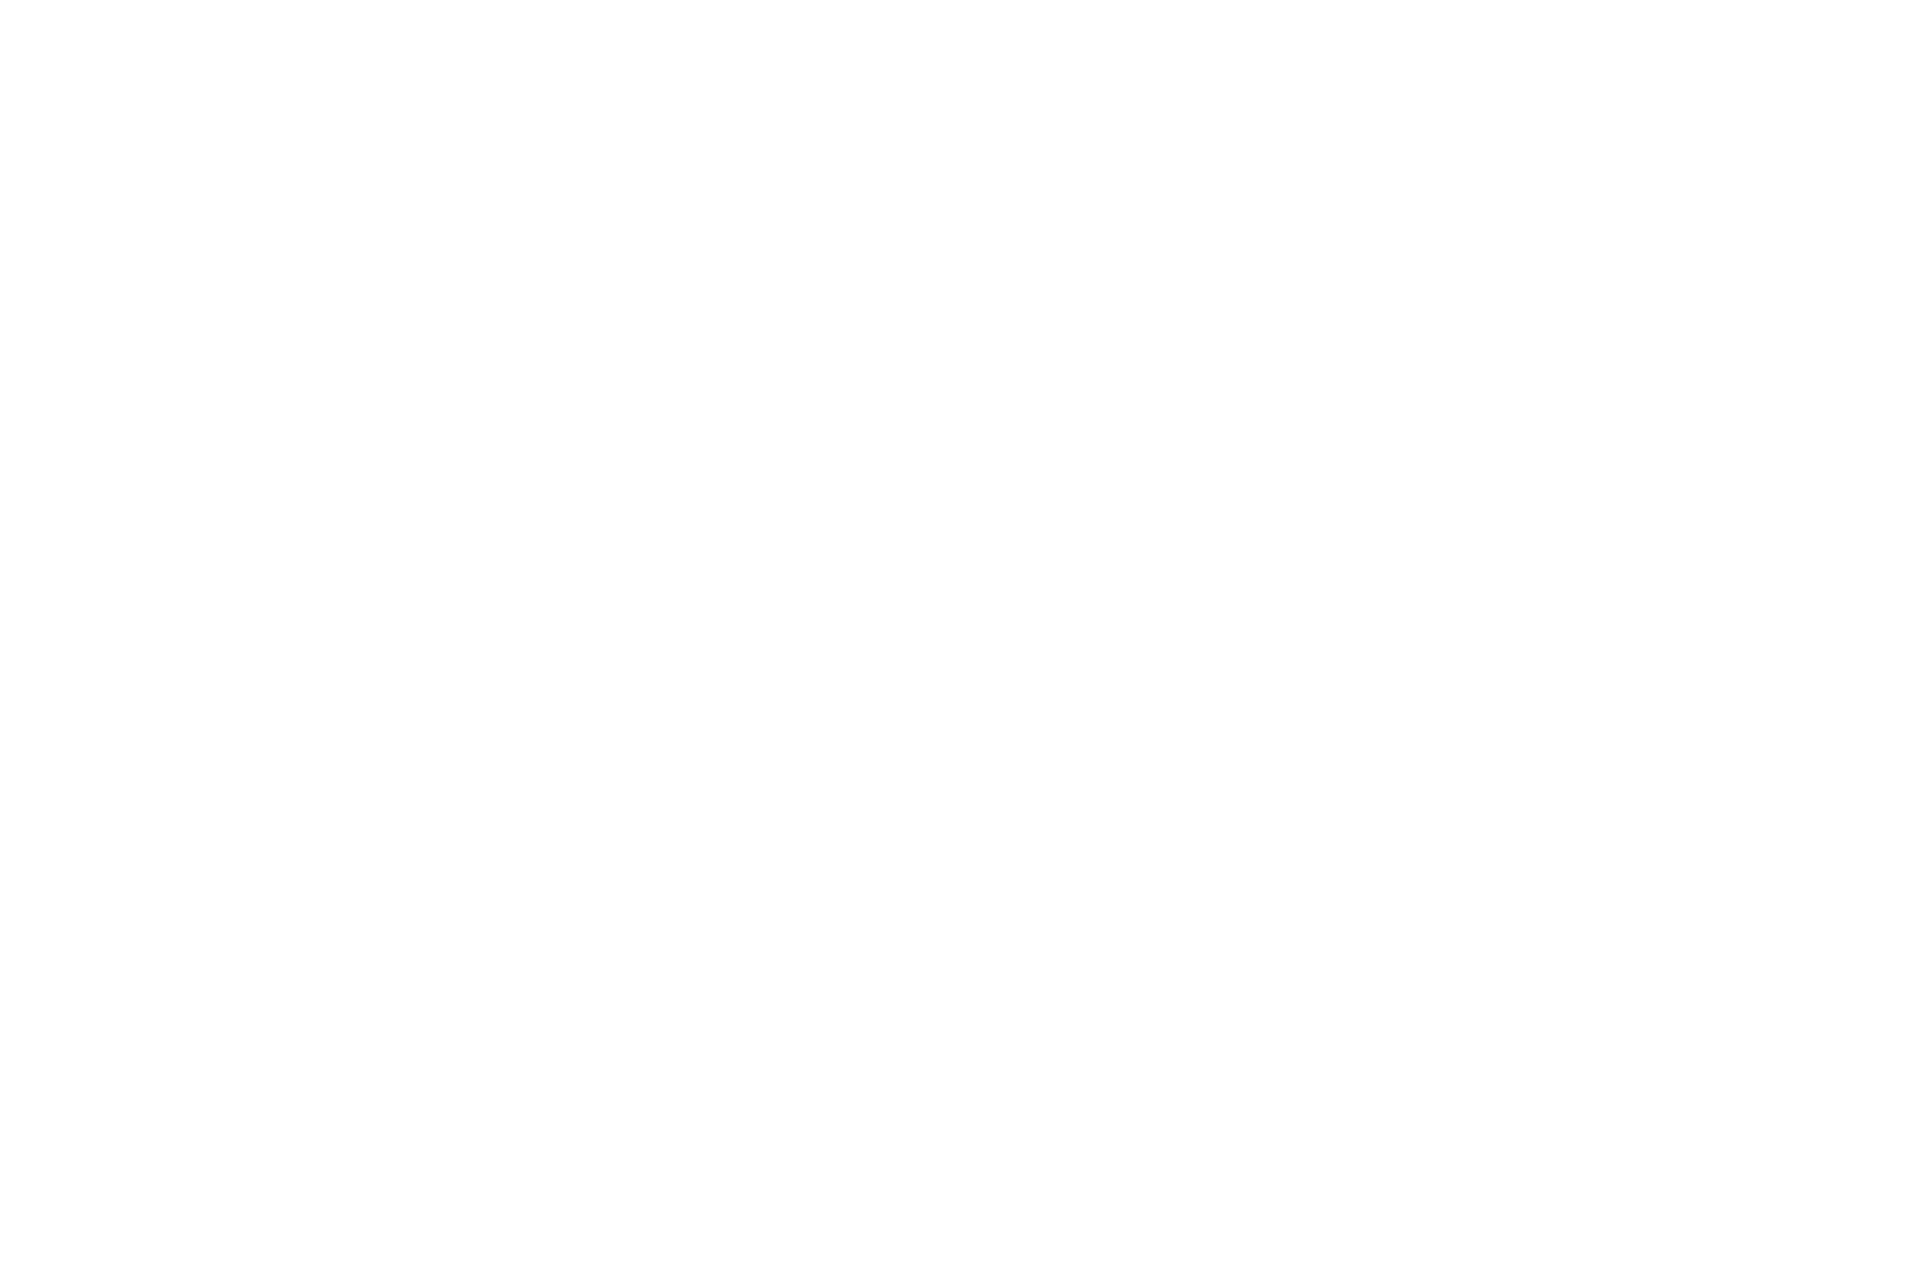
\includegraphics{Hintergruende/Interface_1920x1280px.png}};
	  \end{scope}
	  \fill[gray, path fading=south, fill opacity=.9] (0,-\headheight+3mm) rectangle (\paperwidth, -\headheight);
	\fill[fill=redtext] (0mm,-14mm) rectangle (15mm,-8mm);
	  \end{tikzpicture}
\end{document}